\begin{figure}[hbtp]
  \centering
  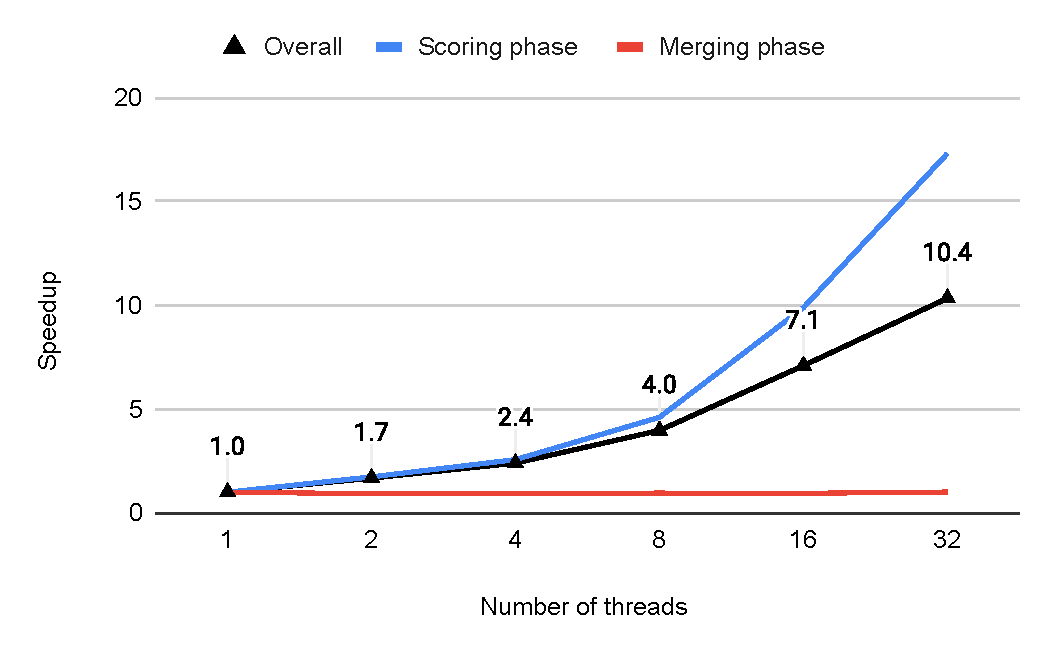
\includegraphics[width=0.98\linewidth]{out/strong-scaling-speedup.pdf} \\[-2ex]
  \caption{Overall speedup of our optimized neighbor-based link predictions methods, and its phases (obtaining edges with top-k scores per thread, and merging scores from each thread into a common scoreboard), on batch sizes of $10^{-2}|E|$, with increasing number of threads (in multiples of 2). Increasing the number of threads causes the merging phase runtime to rise, leading to a speedup below $1$.\ignore{For this plot, we consider the link-prediction methods \textit{HP4}, \textit{LHN4}, \textit{AA4}, and \textit{RA4}, which perform the best overall. Note that the numerical suffix added to the acronym of each link prediction method indicates the \textit{MAX\_MEDIATOR\_DEGREE} parameter setting.}}
  \label{fig:strong-scaling}
\end{figure}
